\chapter{Redis $\to$ Remote Dictionary Server}

\emph{Redis}, acronimo di \emph{Remote Dictionary Server}, é un archivio dati veloce, open source, in memoria e di tipo chiave-valore(\textbf{dbms NoSQL}).
Si basa su una struttura a dizionario: ogni valore immagazzinato é abbinato ad una chiave univoca che ne permette il recupero.
É stato sviluppato nel linguaggio di programmazione C, e funziona principalmente con sistemi unix based, non esiste un supporto ufficiale
per Windows.
Redis si basa su un modello client-server, infatti i programmi esterni dialogano con il server Redis utilizzando un socket TCP e un protocollo specifico
di tipo request-response.
Il client invia una richiesta al server attendendo la risposta sul socket ed il server elabora il comando e
invia la risposta al client.
Inoltre, é possibile interagire con il server anche da linea di comando con un programma chiamato \texttt{redis-cli}, grazie ad esso viene
semplificato notevolmente il lavoro di hacking con il sistema.\\

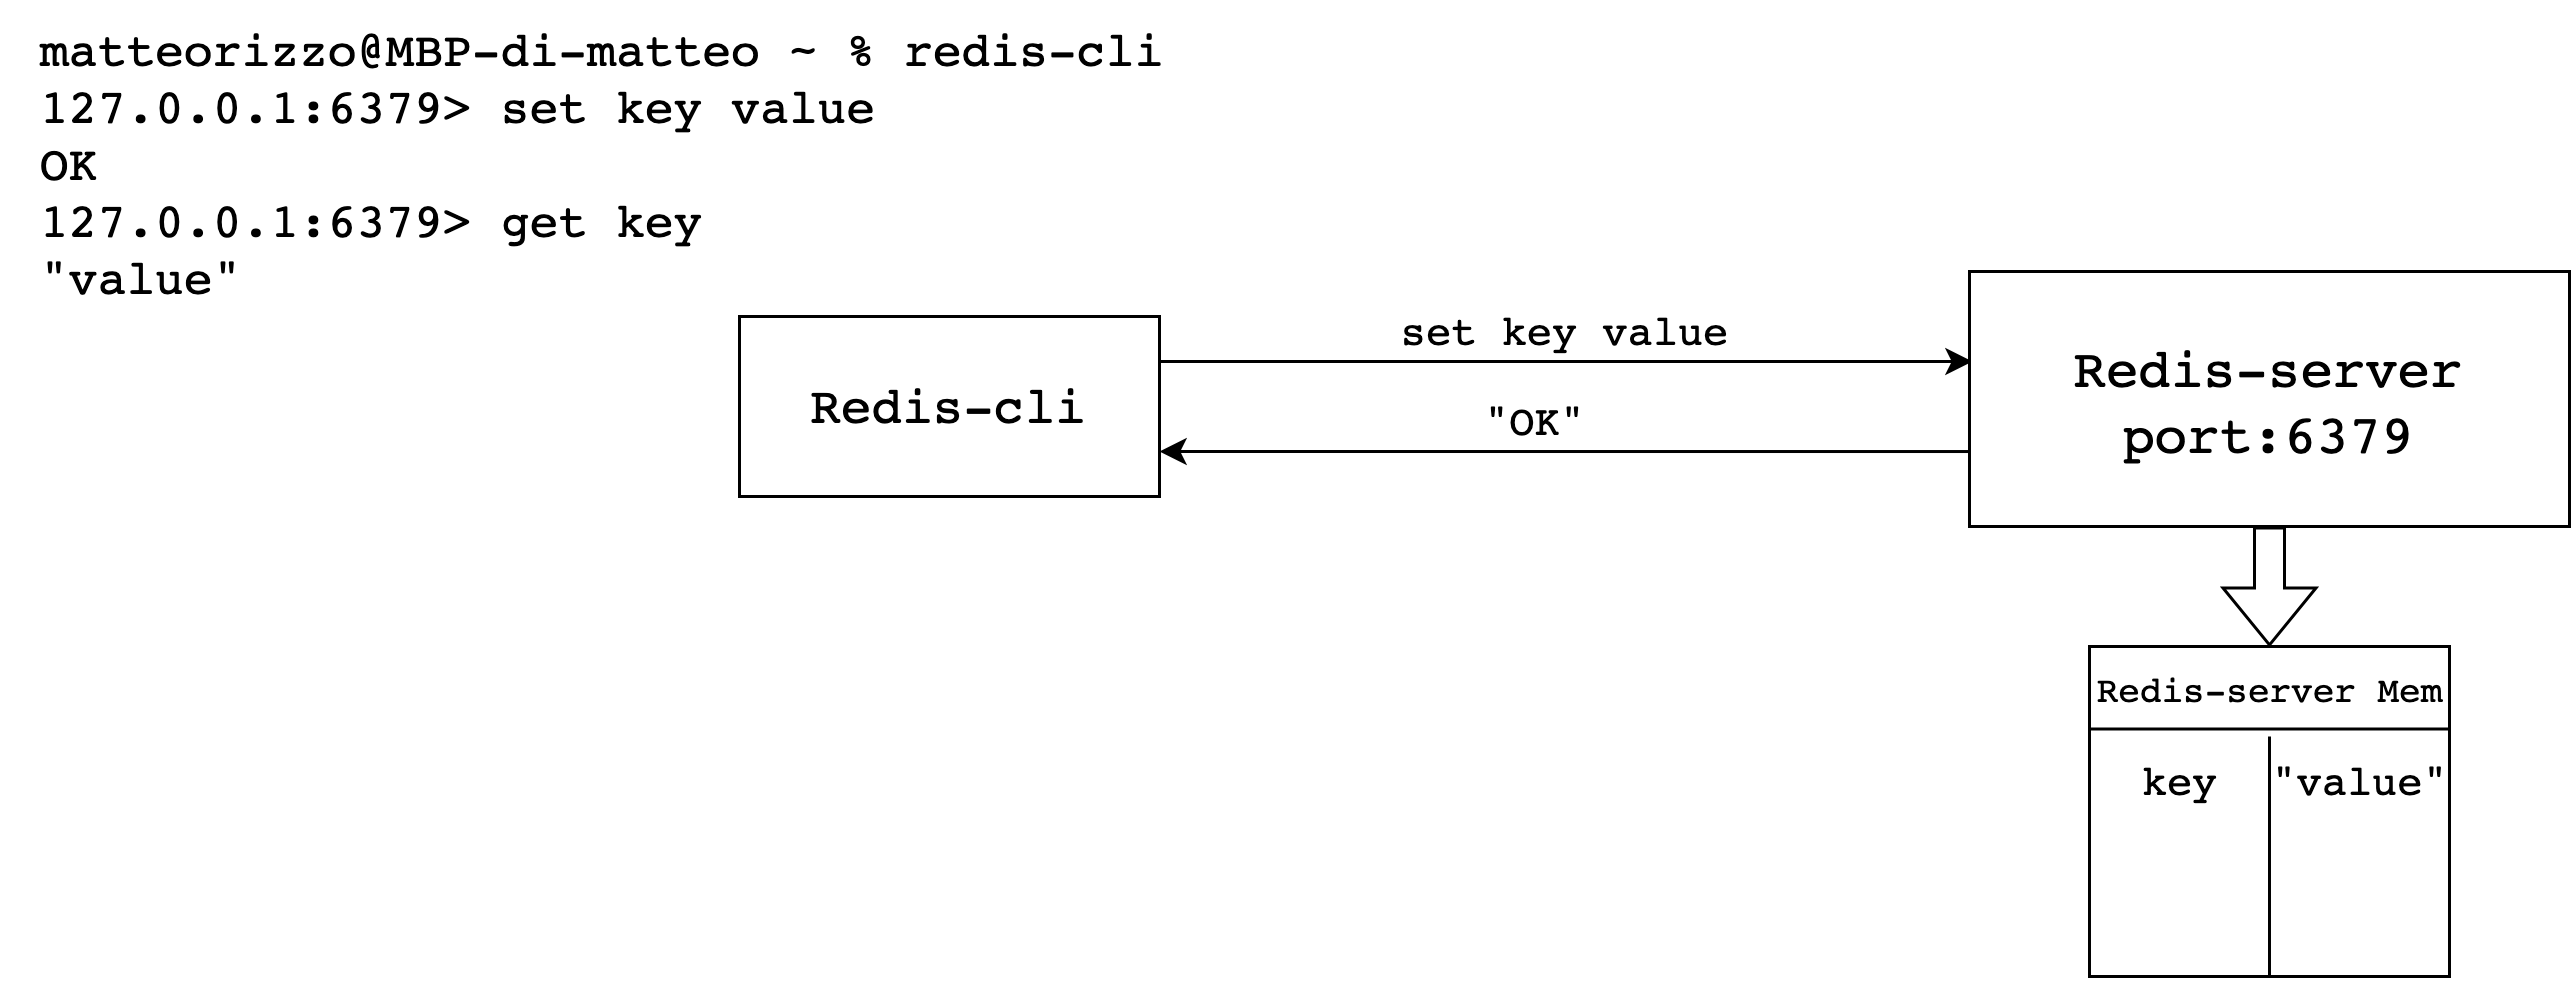
\includegraphics[width=1\textwidth]{img/redisClientServer}

\section{Caratteristiche}
\subsection{Strutture Dati}
Una caratteristica di Redis é mettere a disposizione una grande varietá di tipi di dati associabili alle chiavi, infatti il valore archiviato
in corrispondenza di una certa chiave puó essere molto differente da un tipo semplice come la stringa ed il valore stesso puó addirittura
rappresentare una struttura dati. Inoltre vi é una grandissima possibilitá di manipolazione grazie all'elevato numero di funzioni presenti.
I tipi di dato disponibili sono:
\begin{itemize}
    \item \textbf{Stringhe}: é il tipo piú semplice, vengono memorizzate sequenze di byte, inclusi testo, oggetti serializzati e array binari;
    sono spesso usati per la memorizzazione nella cache;
    \item \textbf{Liste}:rappresentano un elenco di stringhe indicizzate in base all'ordine di inserimento nella struttura. Possono essere
    modificate con inserimenti in testa o in coda. Vi é la possibilitá di trattare una lista come una coda (First In First Out) tramite il comando di inserimento
    \texttt{LPUSH} e il comando di prelievo \texttt{RPOP} oppure puó essere trattata come una pila (First In Last Out) tramite i rispettivi comandi 
    \texttt{LPUSH} e \texttt{LPOP};
    \item \textbf{Set}: é una raccolta non ordinata di stringhe univoche(sono chiamate \emph{membri} del set); quindi vi é la possiblitá
    di utilizzare questa struttura dati per tenere traccia degli elementi univoci, rappresentare relazioni o eseguire operazioni di insiemi
    comuni come intersezioni, unioni e differenze;
    \item \textbf{Hash}: sono oggetti strutturati come raccolte di coppie campo(chiave)-valore. Possono essere utilizzati per rappresentare oggetti
    di base e per memorizzare raggruppamenti di contatori;
    \item \textbf{SortedSet}: sono una versione modificata dei Set. Sono anch'essi insiemi di stringhe che non ammettono duplicati ma, in piú,
    includono un valore detto \texttt{score} associato ad ogni elemento, in base al quale é possibile ordinare in senso ascendento o discendente i valori
    dell'insieme.
\end{itemize}
    Ovviamente associati a queste strutture dati vi sono molti comandi specifici per ognuna, analizzare tutti i comandi non ha molto senso, quindi
    ogni volta che verranno incontrati dei comandi particolari verranno illustrati in quel momento.


\subsection{\emph{proprietá ACID}}
%FIXME: questa introduzione
Nelle basi di dati relazionali ogni transazione gode delle proprietá ACID. in questa sezione l'obiettivo é mettere in evidenza
quali proprietá vengono verificate da questo dbms, se c'é la possibilitá di abilitare/disabilitare certe proprieta e cosí via.

Innanzitutto, bisogna vedere in che modo sono gestite le transazioni in Redis:\\
i comandi utilizzati per le transazioni sono quattro:
\begin{itemize}
    \item \texttt{MULTI}: contrassegna l'inizio di un blocco di transazione, i comandi successivi verranno accodati per l'esecuzione
    \item \texttt{EXEC}: esegue tutti i comandi precedentemente accodati in una transazione e ripristina lo stato di connessione normale;
    \item \texttt{DISCARD}: svuota tutti i comandi precedentemente accodati in una transazione e ripristina lo stato di connessione normale;
    \item \texttt{WATCH}: contrassegna le chiavi fornite con un certo valore per eseguire un controllo condizionale al momento dell'esecuzione
    di una transazione (serve per la gestione di lock, ovvero controllo della concorrenza)
\end{itemize}

Quindi una transazione viene eseguita in questo modo:
\begin{enumerate}
    \item inviamo il comando \texttt{MULTI}. Redis risponde \texttt{OK};
    \item digitiamo i comandi che devono far parte della transazione. Redis risponde \texttt{QUEUED}, ovvero il comando non viene eseguito
    istantaneamente ma viene messo in coda;
    \item conclusione della transazione: si puó scegliere se eseguire tutti i comandi con \texttt{EXEC} oppure annullare la transazione
    con \texttt{DISCARD}.
\end{enumerate}

Di seguito riporto un esempio utilizzando \texttt{redis-cli} con la struttura dati lista, quindi i comandi per gestire le liste in questo esempio
sono 2: \texttt{LPUSH} comando per inserire un singolo elemento nella lista e \texttt{LRANGE} comando per ottenere tutti i valori presenti nella lista

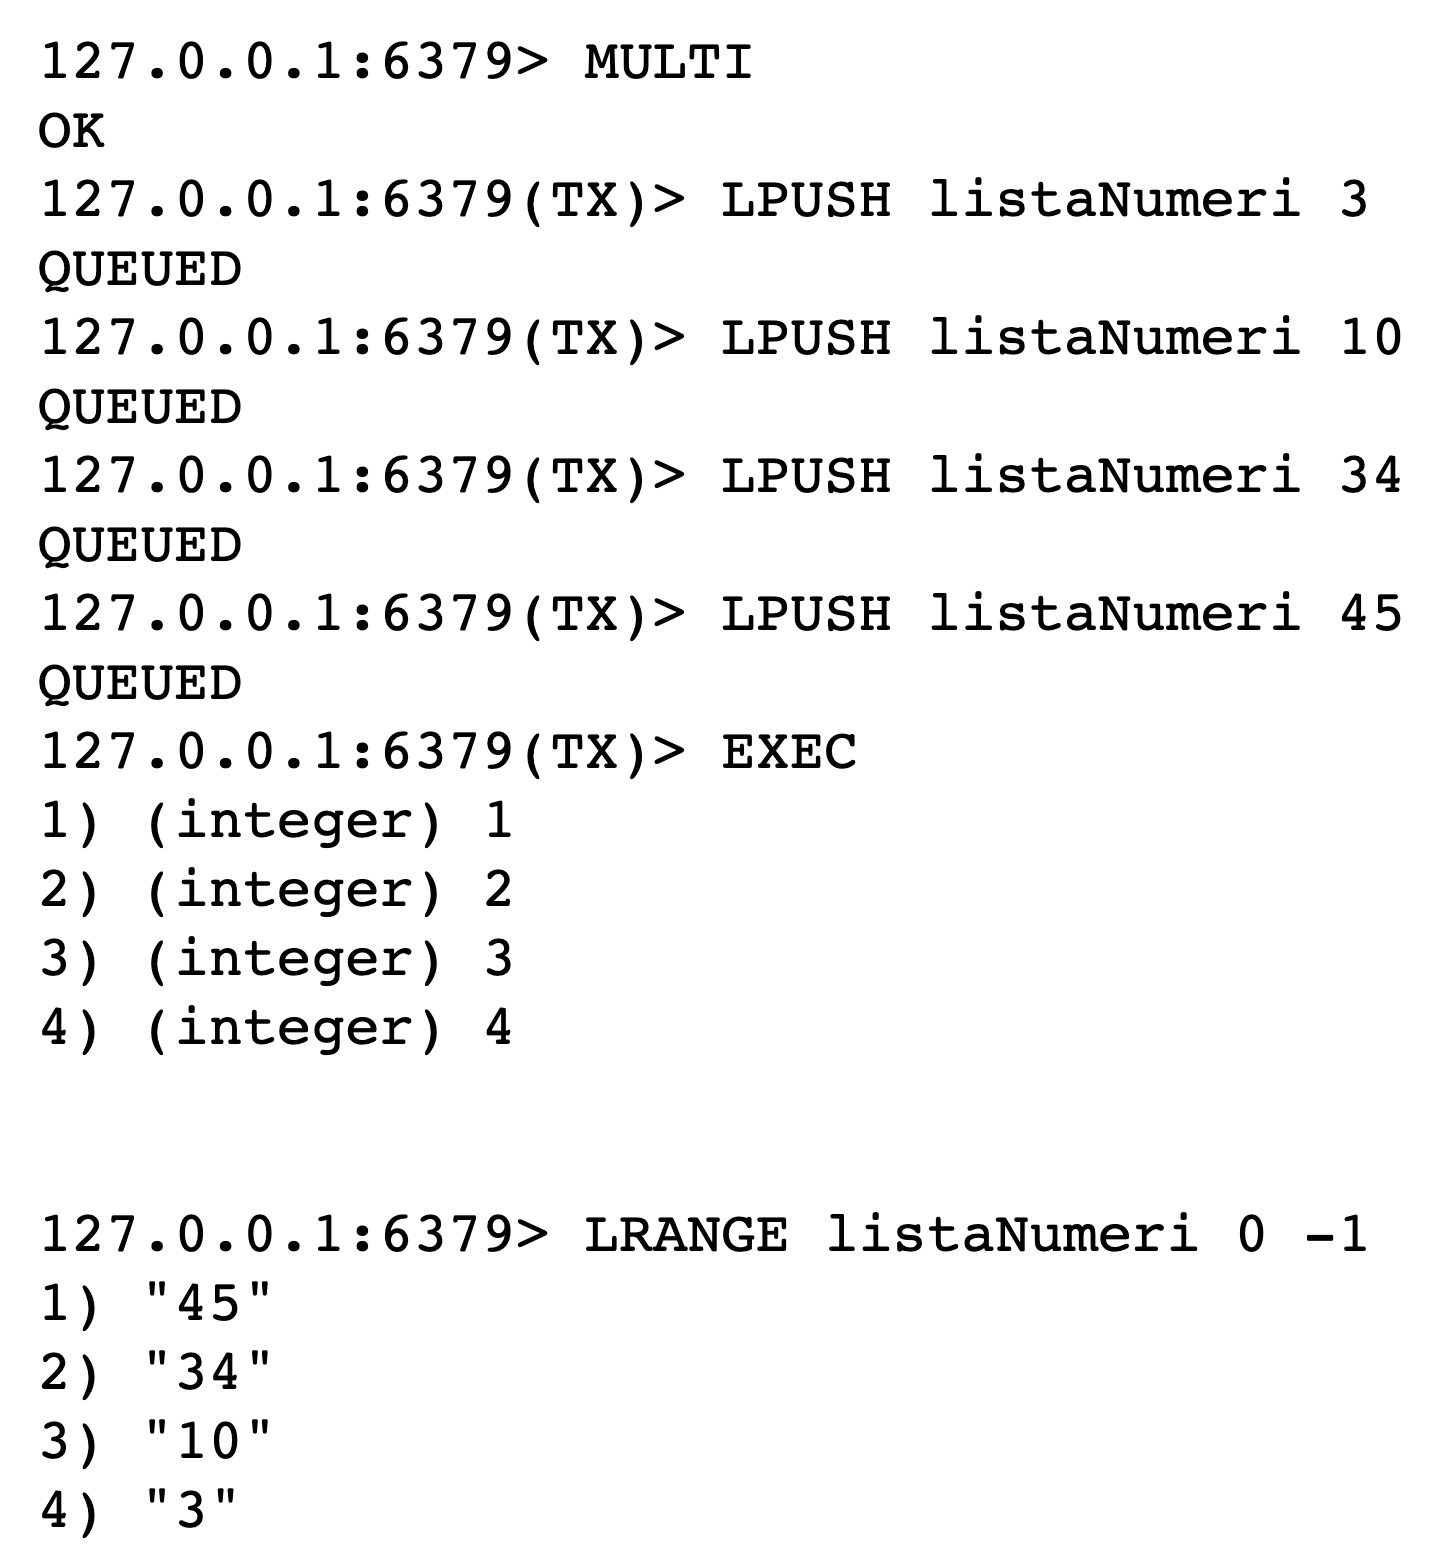
\includegraphics[width=0.7\textwidth]{img/transazioneRedis}\\
Si puó notare come l'inserimento di tutti i valori nella lista avvenga dopo il comando \texttt{EXEC}.\\

Quindi, passando all'illustrazione delle proprietá ACID:
\begin{itemize}
    \item \textbf{Atomicitá}: Redis puó avere due livelli di atomicitá:
      \begin{itemize}
          \item singola operazione: ovvero ogni singola richiesta da parte del client viene eseguita in maniera atomica dal server;
          \item transazione con operazioni multiple: come illustrato sopra con i vari comandi \texttt{MULTI}, \texttt{EXEC} ...;
      \end{itemize}

    \item \textbf{Isolamento}:
    Tutti i comandi in una transazione vengono serializzati ed eseguiti in sequenza. Una richiesta inviata da un altro client
    non sará mai soddisfatta nel bel mezzo dell'esecuzione di una transazione. Ció garantisce che i comandi vengano eseguiti
    come un'unica operazione isolata.\\
    Inoltre, vi é un meccanismo che riesce a fornire delle garanzie aggiuntive, in cui viene fatta una sorta di operazione
    di check-and-set.
    Questo meccanisco utilizza il comando \texttt{WATCH} definito precedentemente.
    Le chiavi, su cui viene definito watch, vengono continuamente monitorate per eventuali modifiche; se anche una sola chiave monitorata
    da \texttt{WATCH }viene modificata prima della \texttt{EXEC}, l'intera transazione verrá abortita.\\

    Consideriamo un esempio in pseudo-codice in cui si deve aumentare il valore di una chiave di 1.

    \begin{lstlisting}[autogobble]
       num = GET sampleKey
       num = num + 1
       SET sampleKey num\end{lstlisting}

    i comandi mostrati sopra funzioneranno senza problemi purché sia presente un solo utente che esegue l'operazione in un determinato momento.\\
    Il problema si verifica nel caso in cui ci siano piú utenti che tentano di aumentare il valore della chiave contemporaneamente.
    Possiamo eliminare questo potenziale problema di race condition utilizzando il comando \texttt{WATCH} nel modo seguente:

    \begin{lstlisting}[autogobble]
       WATCH sampleKey
       num = GET sampleKey
       num = num + 1
       MULTI
       SET sampleKey num
       EXEC\end{lstlisting}

    Con questa implementazione, se si dovesse verificare una race condition ed un client modifica il valore di \texttt{sampleKey} tra il nostro
    \texttt{WATCH} e \texttt{EXEC}, la transazione verrá interrotta. Avremo bisogno di ripetere la transazione quando la race condition non sará
    piú presente.\\
    Quindi questo é un modo efficace per ottenere un buon livello di isolamento a livello di transazioni.

    \item consistenza
    \item persistenza(durability) %parlate anche dei dati salvati in cache, vantaggi/svantaggi che ne derivano
          
\end{itemize}

\subsection{Ambiti di utilizzo}

\subsection{sistema distribuito (cenni)}
%teorema cap, proprietá base





%Le principali caratteristiche sono la velocitá e la struttura semplice dei database. Infatti, i dati vengono scritti direttamente sulla
%memoria RAM del server e possono essere richiamati molto piú velocemente rispetto ad altri database.
